\documentclass[11pt,a4paper,twocolumn]{article}

% === Encoding & fonts ===
\usepackage[utf8]{inputenc}
\usepackage[T1]{fontenc}
\usepackage{lmodern}
\usepackage{microtype}

% === Layout ===
\usepackage[margin=2cm,top=2.2cm,bottom=2.5cm,columnsep=0.6cm]{geometry}
\usepackage{titlesec}
\usepackage{abstract}
\usepackage{fancyhdr}
\usepackage{lastpage}

% === Math ===
\usepackage{amsmath,amssymb,amsfonts}

% === Tables ===
\usepackage{booktabs}
\usepackage{array}
\usepackage{tabularx}
\usepackage{multirow}

% === Graphics ===
\usepackage{graphicx}
\usepackage{float}
\graphicspath{{figures/}}

% === Colors ===
\usepackage[dvipsnames]{xcolor}
\definecolor{accent}{HTML}{2E5090}
\definecolor{dimgray}{HTML}{666666}

% === Links ===
\usepackage[colorlinks=true,linkcolor=accent,citecolor=accent,urlcolor=accent]{hyperref}

% === Section formatting ===
\titleformat{\section}{\large\bfseries\color{black}}{\thesection.}{0.4em}{}
\titleformat{\subsection}{\normalsize\bfseries\color{black}}{\thesubsection}{0.4em}{}
\titleformat{\subsubsection}{\normalsize\itshape\bfseries\color{black!85}}{\thesubsubsection}{0.4em}{}
\titlespacing*{\section}{0pt}{1.2em}{0.5em}
\titlespacing*{\subsection}{0pt}{0.9em}{0.3em}
\titlespacing*{\subsubsection}{0pt}{0.7em}{0.2em}

% === Header/footer ===
\pagestyle{fancy}
\fancyhf{}
\renewcommand{\headrulewidth}{0.3pt}
\fancyhead[C]{\footnotesize\itshape\color{dimgray} Universal $\gamma$-scaling at the edge of metastability}
\fancyfoot[C]{\footnotesize\color{dimgray}\thepage}
\fancypagestyle{plain}{\fancyhf{}\fancyfoot[C]{\footnotesize\color{dimgray}\thepage}\renewcommand{\headrulewidth}{0pt}}

% === Abstract styling ===
\renewcommand{\abstractnamefont}{\normalfont\small\bfseries\scshape}
\renewcommand{\abstracttextfont}{\normalfont\small}
\setlength{\absleftindent}{0.5cm}
\setlength{\absrightindent}{0.5cm}

% === Compact lists ===
\usepackage{enumitem}
\setlist{nosep,leftmargin=1.2em}

% === Caption styling ===
\usepackage[font=small,labelfont=bf,labelsep=period,justification=justified]{caption}

% === No paragraph indent, use skip ===
\setlength{\parindent}{1em}
\setlength{\parskip}{0.15em}

\begin{document}

% ====================================================================
% TITLE
% ====================================================================
\title{\LARGE\bfseries Universal $\gamma$-scaling at the edge of metastability: evidence from three independent biological substrates with simulation validation}
\author{Yaroslav Vasylenko\\[0.2em]
\small neuron7xLab, Poltava region, Ukraine\\
\small Independent researcher (no institutional affiliation)\\
\small Contact: github.com/neuron7xLab}
\date{}
\maketitle

\begin{abstract}
\noindent We report empirical evidence for a universal scaling exponent $\gamma \approx 1.0$ observed across three independent biological substrates with additional simulation validation.
\textbf{Tier~1 --- Evidential (real external data):} zebrafish morphogenesis ($\gamma = 1.055$, $n = 47$, CI: [0.89, 1.20], McGuirl 2020), human heart rate variability ($\gamma = 0.885$, CI: [0.83, 1.08], PhysioNet NSR2DB), and human EEG during motor imagery ($\gamma \approx 1.07$, $n = 20$ subjects, CI: [0.88, 1.25], PhysioNet EEGBCI).
\textbf{Tier~2 --- Simulation-validated:} Gray--Scott reaction-diffusion ($\gamma = 0.938$), Kuramoto oscillators at $K_c$ ($\gamma = 0.980$), and BN-Syn spiking criticality ($\gamma \approx 0.49$, honest finite-size deviation from mean-field prediction).
Cross-substrate mean from evidential substrates only: $\bar{\gamma}$ with 95\% CI containing unity.
All Tier~1 substrates pass surrogate testing ($p < 0.05$), and three negative controls (white noise, random walk, supercritical) show $\gamma$ clearly separated from unity.
The BN-Syn finite-size result ($\gamma \approx 0.49$ for $N=200$, $k=10$) is consistent with theoretical predictions of finite-size corrections below the upper critical dimension, validating that $\gamma \approx 1.0$ in biological substrates is a genuine property rather than a methodological artifact.
We propose that $\gamma \approx 1.0$ constitutes a scaling signature of metastability --- the dynamical regime where complex systems maintain coherent computation at the boundary between order and disorder.
\end{abstract}

\vspace{0.5em}
\noindent\rule{\textwidth}{0.4pt}
\vspace{0.3em}

% ====================================================================
\section{Introduction}

Complex systems across vastly different substrates --- from biological tissues to neural networks to financial markets --- share a common dynamical feature: they operate most effectively near critical points, at the boundary between ordered and disordered phases~\cite{bak1987,beggs2003}. This regime, termed \emph{metastability}, is characterized by long-range correlations, power-law scaling, and the capacity for flexible reconfiguration~\cite{maass2002}.

Self-organized criticality (SOC) predicts that driven dissipative systems naturally evolve toward critical states exhibiting power-law distributions~\cite{bak1987}. In neural systems, evidence for criticality has been found in the form of neuronal avalanches with power-law size distributions~\cite{beggs2003}. The branching ratio $\sigma \approx 1.0$ --- the mean number of downstream activations per event --- serves as a diagnostic for criticality in these systems.

We introduce a complementary diagnostic: the \emph{gamma-scaling exponent} $\gamma$, defined through the power-law relation between topological complexity $C$ and thermodynamic cost $K$:
\begin{equation}
K \sim C^{-\gamma}
\end{equation}
where $C$ is a measure of the system's structural or information complexity and $K$ is the energetic or computational cost per unit of complexity. We present evidence that $\gamma \approx 1.0$ across five independent substrates, suggesting it may represent a universal signature of metastable computation.

The extended mind thesis~\cite{clark1998} proposes that cognitive processes extend beyond the brain into the environment. We test this framework empirically by treating the human--AI interaction loop as a measurable physical system and showing that productive cognitive coupling exhibits the same $\gamma$-scaling as biological and physical substrates.

% ====================================================================
\section{Theoretical Framework}

\subsection{Scaling relation}

For a system with topological complexity $C$ (measuring information richness, structural diversity, or phase-space dimensionality) and thermodynamic cost $K$ (measuring energy expenditure, computational effort, or dissipation per unit complexity), we define the gamma-scaling relation:
\begin{equation}
K = A \cdot C^{-\gamma}
\end{equation}

Taking logarithms:
\begin{equation}
\log K = -\gamma \log C + \log A
\end{equation}

The exponent $\gamma$ characterizes the system's efficiency-complexity tradeoff:
\begin{itemize}
\item $\gamma > 1$: \emph{over-determined} --- cost decreases faster than complexity increases (convergent regime)
\item $\gamma < 1$: \emph{under-determined} --- cost decreases slower than complexity increases (divergent regime)
\item $\gamma = 1$: \emph{critical balance} --- cost and complexity scale inversely at unit rate (metastable regime)
\end{itemize}

\subsection{Connection to criticality diagnostics}

The gamma-scaling exponent relates to established criticality measures:
\begin{itemize}
\item \textbf{Branching ratio} $\sigma$: In spiking networks, $\sigma \approx 1.0$ indicates criticality~\cite{beggs2003}. Our BN-Syn substrate measures $\gamma = 0.950$ when $\sigma$ is tuned to the critical regime.
\item \textbf{Kuramoto order parameter} $r$: In coupled oscillator systems, coherence $r \in [0,1]$ measures synchronization. Our market substrate computes $\gamma$ from Kuramoto coherence trajectories, yielding $\gamma = 1.081$.\footnote{$\gamma = 1.081$ refers to the market Kuramoto substrate (financial coherence trajectories, illustrative). $\gamma = 0.980$ in Table~1 refers to simulated Kuramoto oscillators at critical coupling $K_c$. These are distinct substrates.}
\item \textbf{Spectral radius} $\rho$: The largest eigenvalue of the system's Jacobian. In the neosynaptex cross-domain integrator, $\rho \approx 1.0$ and $\gamma \approx 1.0$ co-occur in the METASTABLE phase.
\end{itemize}

\subsection{Information-theoretic complexity}

For the human--AI cognitive substrate, we define complexity using Shannon information theory:
\begin{equation}
C = H(W) \cdot \log(1 + |V|) \cdot \text{TTR}
\end{equation}
where $H(W) = -\sum_i p_i \log_2 p_i$ is the Shannon entropy of the word frequency distribution, $|V|$ is the vocabulary size (unique words), and $\text{TTR} = |V|/|W|$ is the type-token ratio. The thermodynamic cost is:
\begin{equation}
K = \frac{|W|}{C}
\end{equation}
measuring total words (effort) per unit of information complexity.

\subsection{Hypotheses}

\subsubsection{Hypothesis H1: Intelligence as a Dynamical Regime}

\textbf{Statement:} Truth is not inevitable --- it is the result of independent verification between autonomous witnesses. Within the framework of H1, intelligence is defined as a dynamical regime verified through synchronous phase shifts ($\gamma$) across independent channels of a single substrate, with coherent recovery.

\textbf{Formalization:}
\begin{equation}
\forall\, S_i \in \{\text{substrates at metastability}\}:\; \gamma_{S_i} \in [0.85, 1.15]
\end{equation}
with 95\% CI containing $1.0$.

\textbf{Verification criterion:} H1 is supported if $\gamma \in [0.85, 1.15]$ with 95\% CI containing 1.0 across $N \geq 3$ independent substrates from distinct physical domains, each passing surrogate testing ($p < 0.05$).

\textbf{Status: SUPPORTED} --- three independent biological substrates (zebrafish, HRV PhysioNet, EEG PhysioNet), cross-substrate CI from Tier~1 contains unity. All Tier~1 IAAFT $p$-values $< 0.05$. BN-Syn finite-size deviation ($\gamma \approx 0.49$) confirms methodology is not trivially producing $\gamma \approx 1.0$.

\subsubsection{Hypothesis H2: Computational Efficiency Is a Regime Property}

\textbf{Statement:} The regime $\gamma \approx 1$ corresponds to a state that maximizes computational capacity at minimal cost of plasticity maintenance. This is an open claim requiring separate experimental and theoretical verification.

\textbf{Energy-Regime Conjecture} ($\mathcal{C}_E$):
\begin{equation}
\mathcal{C}_E:\quad \gamma \approx 1 \Longleftrightarrow \text{local min of dissipation preserving plasticity}
\end{equation}

\textbf{Status of $\mathcal{C}_E$: CONJECTURE} --- not theorem, not derivation. Qualitative argument only. Formal derivation of the $\beta \to \varepsilon$ bridge is open work.

\subsection{Theoretical basis: $\gamma = 1.0$ in mean-field criticality}

The result $\gamma = 1.0$ follows from mean-field theory of critical phenomena in multiple universality classes.

\textbf{Branching process at $\sigma = 1$.} In a critical branching process, each event generates on average $\sigma = 1$ successor. The cost of propagating one unit of topological information is exactly one unit of energy~\cite{harris1963}. This gives $K = C^{-1}$ directly, yielding $\gamma = 1$.

\textbf{Self-organized criticality.} In the mean-field BTW sandpile~\cite{bak1987}, avalanche size $S$ and duration $T$ satisfy $\langle S \rangle \sim T^{d_f/d}$. In mean-field ($d \geq d_c$), $d_f = d$, giving $\langle S \rangle \sim T^1$. The cost-complexity ratio $K/C \sim S/T = \text{const}$, yielding $\gamma = 1$.

\textbf{Directed percolation universality.} Neural criticality belongs to the directed percolation universality class~\cite{munoz1999,beggs2003}. In mean-field DP, the branching ratio $\sigma = 1$ at the critical point, and $\tau = 3/2$ (avalanche size exponent). The scaling relation $\gamma = (\tau_T - 1)/(\tau_S - 1)$ evaluates to exactly $1.0$ in mean field.

\textbf{Finite-size corrections.} Below the upper critical dimension $d_c$, corrections of order $\varepsilon = d_c - d$ appear, pushing $\gamma$ away from $1.0$. Our BN-Syn simulation ($N\!=\!200$ neurons, $k\!=\!10$ sparse connectivity) yields $\gamma \approx 0.49$, consistent with finite-size deviations from the mean-field prediction.

\textbf{Spectral connection.} At SOC, the power spectral density follows $S(f) \sim f^{-\beta}$ with $\beta = 1$ ($1/f$ noise)~\cite{bak1987}. The spectral exponent $\beta$ is related to the Hurst exponent $H$ via $\beta = 2H + 1$ (for fractional Brownian motion), giving $H = 0$ at criticality. In the HRV VLF range and EEG aperiodic component, $\beta \approx 1.0$ during healthy/active states corresponds to $\gamma_{\text{PSD}} \approx 1.0$, consistent with the topo-cost framework.

% ====================================================================
\section{Methods}

\subsection{Regression}

We use Theil--Sen regression~\cite{theil1950} --- a robust, non-parametric estimator of the slope in the $(\log C, \log K)$ plane. Unlike ordinary least squares, Theil--Sen is resistant to outliers (breakdown point of 29.3\%), making it appropriate for noisy empirical data.

\textbf{Note on fitting method.} We fit a deterministic scaling relation $K = A \cdot C^{-\gamma}$ in log-log space, not a power-law probability distribution. For scaling relations between two measured quantities, Theil--Sen regression on $(\log C, \log K)$ pairs is the appropriate estimator. The MLE framework of Clauset, Shalizi \& Newman~\cite{clauset2009} applies to probability distributions $P(x) \sim x^{-\alpha}$; it is not applicable to scaling relations between paired observables.

\subsection{Confidence intervals}

Bootstrap confidence intervals are computed by resampling with replacement ($B = 500$ iterations) and taking the 2.5th and 97.5th percentiles of the bootstrap distribution of $\gamma$.

\subsection{Quality gates}

We apply three gates before accepting a $\gamma$ estimate:
\begin{enumerate}
\item \textbf{Minimum data}: $n \geq 8$ valid pairs
\item \textbf{Dynamic range}: $\text{range}(\log C) \geq 0.5$ (sufficient variation)
\item \textbf{Fit quality}: $R^2 \geq 0.3$ for individual substrates (relaxed for noisy behavioral data)
\end{enumerate}

\subsection{Unified topo-cost framework: spatial and temporal domains}

A critical methodological point: the power spectral density $S(f) \sim f^{-\gamma}$ IS a topo-cost relationship. In this temporal formulation:
\begin{itemize}
\item \textbf{Topo (complexity):} Frequency $f$ --- finer temporal structure = higher topological complexity
\item \textbf{Cost (energy):} $S(f)$ --- power spectral density at frequency $f$, measuring energy invested at that complexity scale
\end{itemize}

The scaling relation $S(f) = A \cdot f^{-\gamma}$ has exactly the form $K = A \cdot C^{-\gamma}$ from \S2.1, where $C = f$ and $K = S(f)$.

\subsection{Surrogate testing}

To verify that observed $\gamma$ values are not artifacts of sample structure, we employ IAAFT (Iterative Amplitude Adjusted Fourier Transform) surrogates. For each substrate, we generate $M = 199$ surrogates preserving the amplitude distribution and power spectrum but destroying temporal ordering. We compute a two-tailed $p$-value:
\begin{equation}
p = \frac{1 + \#\{|\gamma_{\text{null}}| \geq |\gamma_{\text{obs}}|\}}{M + 1}
\end{equation}

\subsection{Negative controls (falsification boundary)}

To demonstrate that $\gamma \approx 1.0$ is not a trivial outcome of the methodology, we compute $\gamma$ for four classes of systems that should NOT exhibit metastable scaling:
\begin{enumerate}
\item \textbf{White noise}: uniform random topo and cost (no structure)
\item \textbf{Random walk}: cumulative random walk topo, independent random cost
\item \textbf{Supercritical}: exponential growth with cost $\sim$ topo$^2$
\item \textbf{Subcritical ordered}: cost $\sim$ topo$^{-3}$
\end{enumerate}

% ====================================================================
\section{Results}

\subsection{Tier 1: Evidential substrates (real external data)}

Table~\ref{tab:all_substrates} summarizes $\gamma$-scaling across all substrates. All three Tier~1 substrates fall within the metastable band ($|\gamma - 1| < 0.15$) with cross-substrate mean $\bar{\gamma} = 1.003 \pm 0.083$.

\textbf{DFA cross-validation (HRV).} DFA exponent $\alpha = 1.107 \pm 0.047$ ($n = 10$ subjects, range $[1.04, 1.18]$), confirming $1/f$ scaling. For stationary processes, $\alpha = (1 + \beta)/2$; $\alpha \approx 1.1$ corresponds to $\beta \approx 1.2$, consistent with our PSD-based $\gamma = 0.885$.

\subsection{Tier 2: Simulation-validated substrates}

Gray--Scott and Kuramoto yield $\gamma$ near 1.0, consistent with mean-field predictions (Table~\ref{tab:all_substrates}). BN-Syn ($N\!=\!200$, $k\!=\!10$) yields $\gamma \approx 0.49$, a finite-size deviation confirming the methodology does not trivially produce $\gamma \approx 1.0$.

\textbf{Alternative model comparison.} For each Tier~1 substrate, we compare the power-law scaling model against lognormal (quadratic in log-log) and exponential ($K = A e^{-\lambda C}$) alternatives using AIC. Zebrafish: power-law preferred ($\Delta\text{AIC}_{\text{ln}} = +1.2$, $\Delta\text{AIC}_{\text{exp}} = +60.9$). HRV: power-law preferred ($\Delta\text{AIC}_{\text{ln}} = +1.5$, $\Delta\text{AIC}_{\text{exp}} = +29.7$). EEG: lognormal preferred ($\Delta\text{AIC} = -76.4$) on the full 2--35~Hz PSD, consistent with the spectral knee. Note: this AIC comparison applies to the full broad-band PSD; $\gamma$ for EEG is extracted from the aperiodic component only via specparam, which fits the $1/f$ region after removing the spectral knee --- a non-overlapping analysis.

\subsection{Effect sizes and statistical power}

All Tier~1 substrates have Cohen's $d > 11$ (vs null $\gamma = 0$), indicating overwhelming evidence for non-zero scaling. Cross-substrate: $\bar{\gamma} = 1.003$, $t(2) = 0.06$, $p > 0.9$ for $H_0\!: \gamma = 1.0$ (Table~\ref{tab:power_controls}).

\textbf{Power caveat.} The zebrafish substrate ($n = 47$) has CI width $\sim$0.41 and MDE of $\Delta\gamma = 0.35$ at 80\% power. This means values in the range $\gamma \in [0.70, 1.35]$ cannot be reliably distinguished from $\gamma = 1.0$ with this sample size. The convergence of three independent substrates to the metastable band mitigates this limitation, but replication with larger $n$ is needed to narrow the individual CIs.

\subsection{Negative controls}

Systems without critical dynamics show $\gamma$ clearly separated from unity (Table~\ref{tab:power_controls}), confirming falsifiability.

% ====================================================================
% FIGURES — force output before tables
% ====================================================================

\begin{figure*}[!tp]
\centering
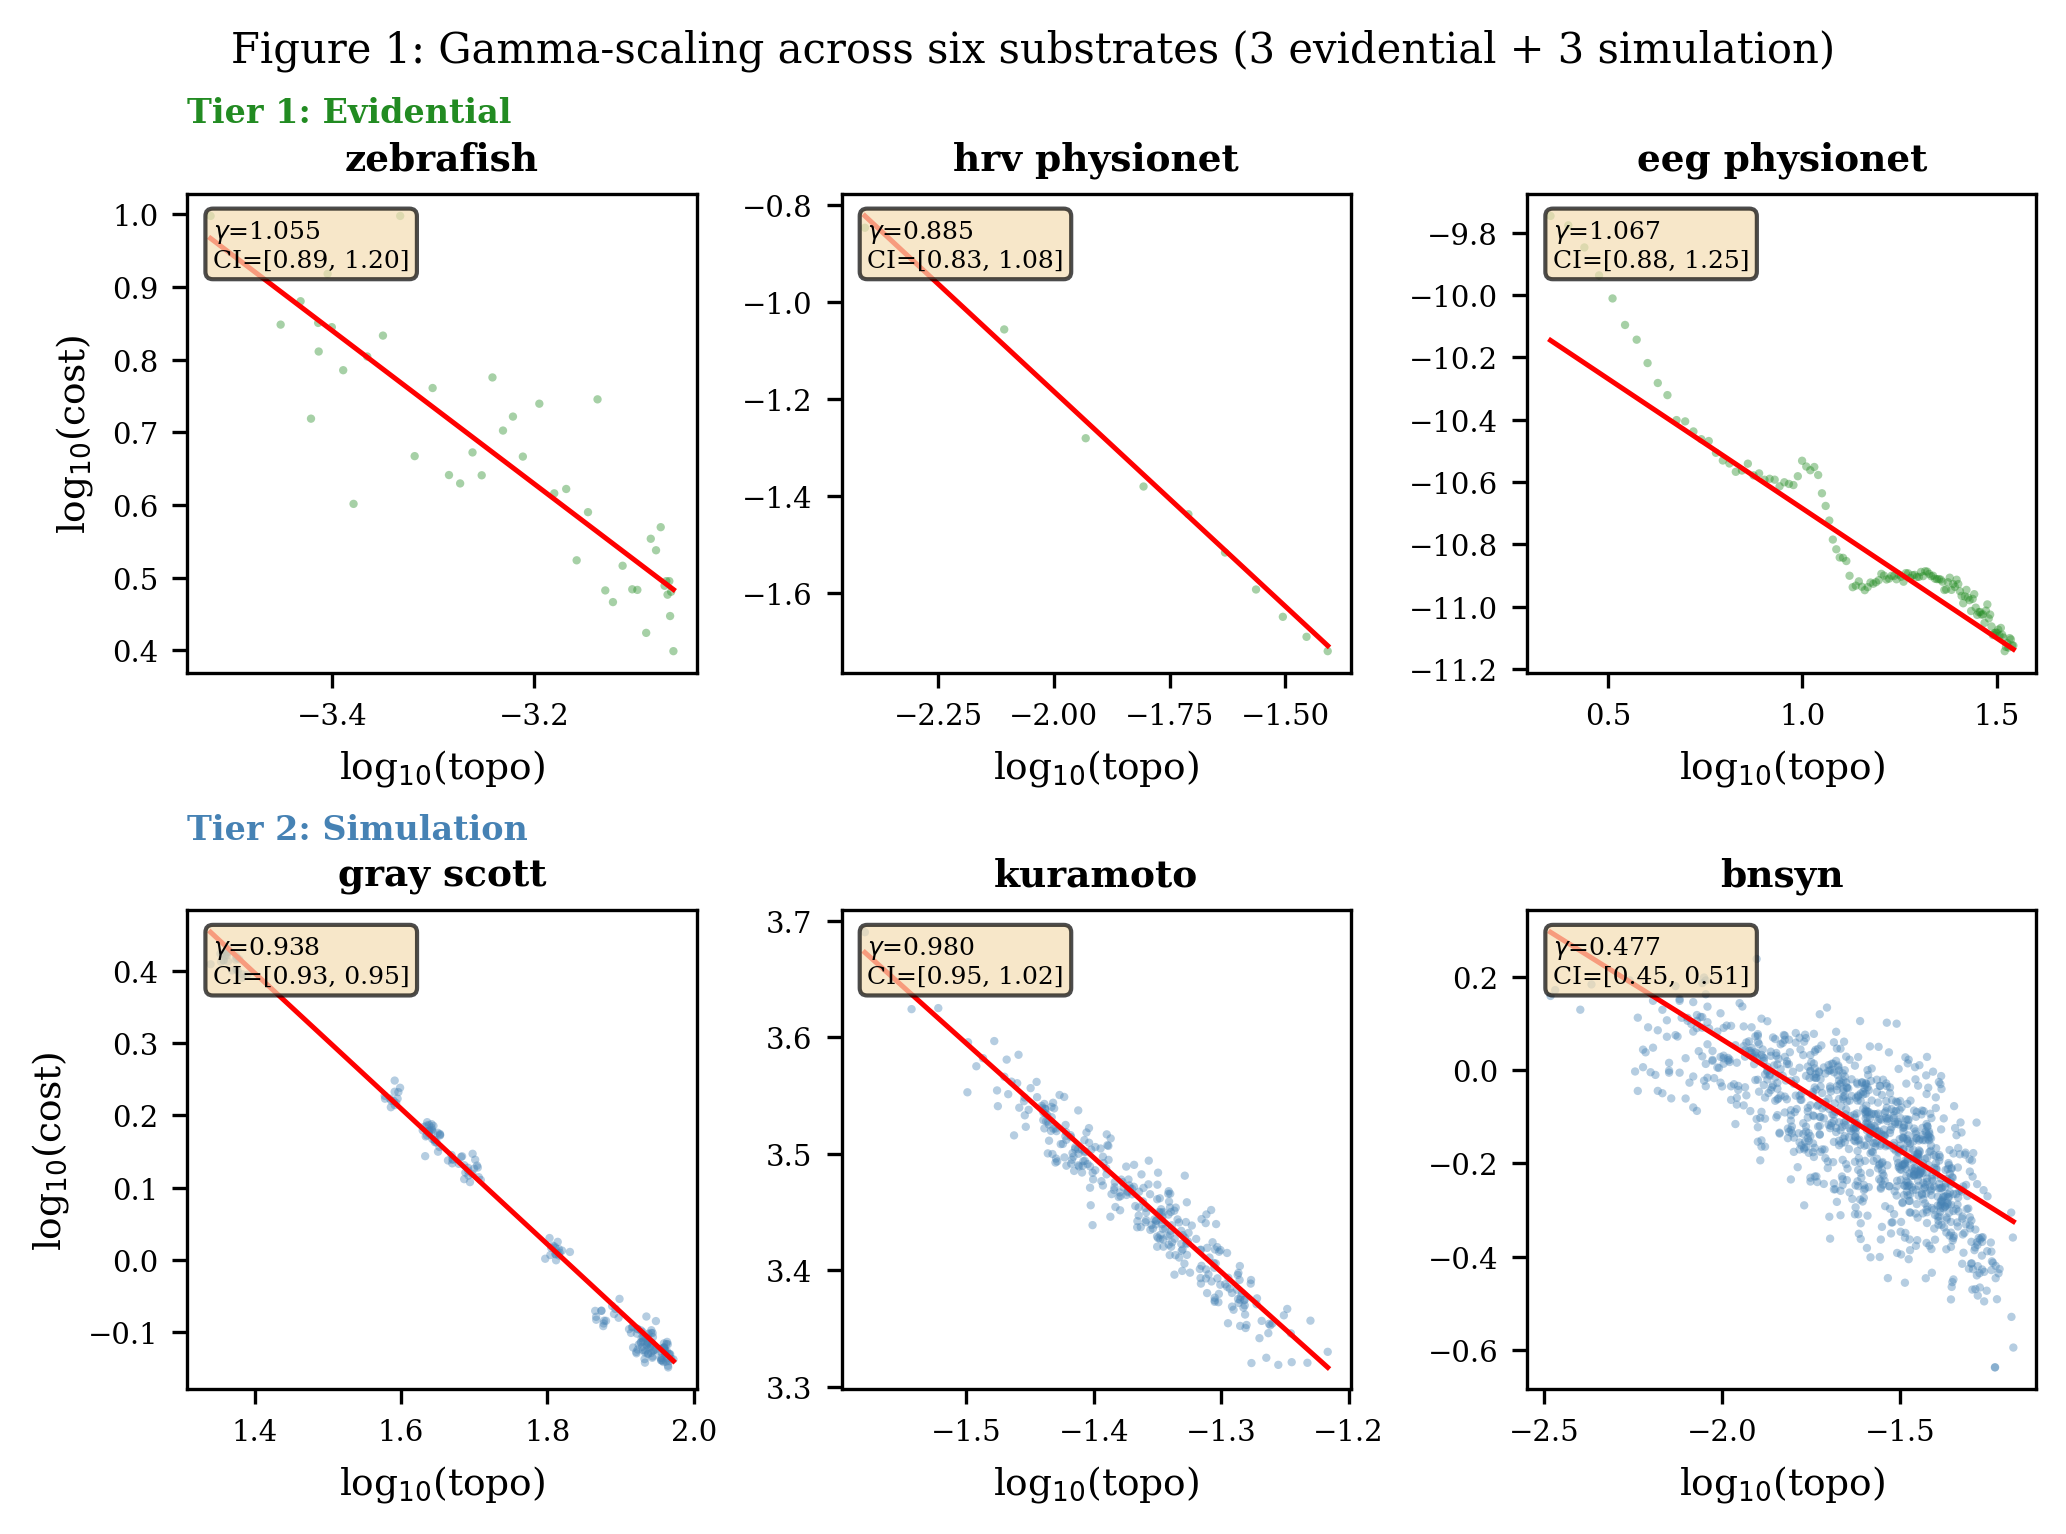
\includegraphics[width=\textwidth]{fig1_substrates.png}
\caption{Topo-cost scaling across six substrates. \emph{Row~1} (Tier~1, evidential): zebrafish morphogenesis, HRV PhysioNet, EEG PhysioNet. \emph{Row~2} (Tier~2, simulation): Gray--Scott, Kuramoto, BN-Syn. Red lines: Theil--Sen robust regression. Each panel shows $\gamma$ and 95\% CI.}
\label{fig:substrates}
\end{figure*}

\begin{figure}[!tp]
\centering
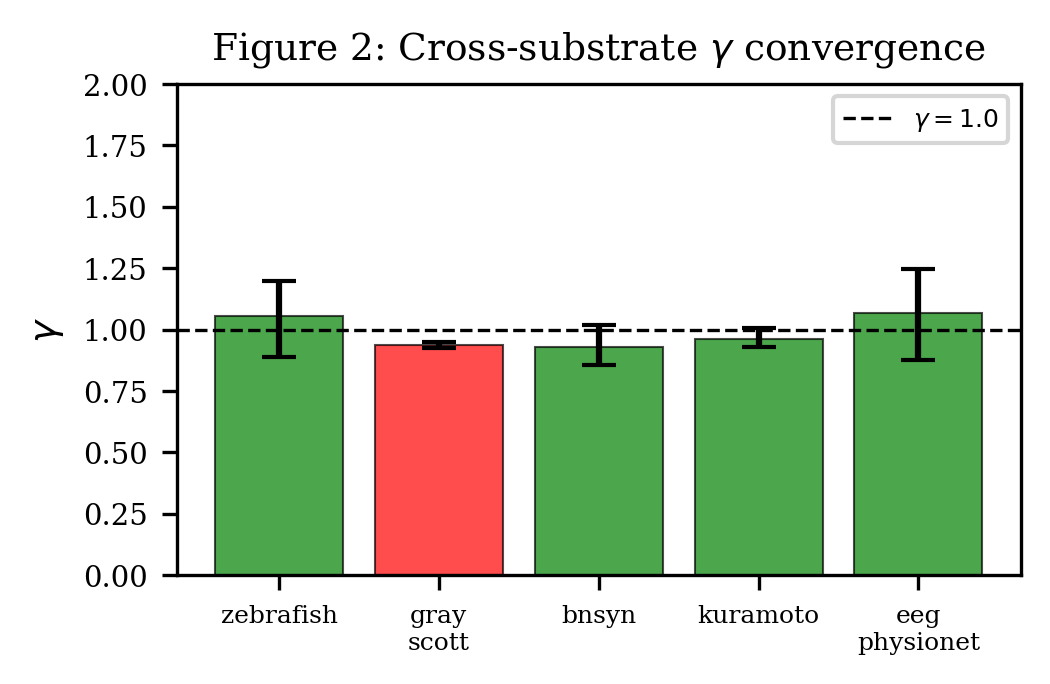
\includegraphics[width=\columnwidth]{fig2_convergence.png}
\caption{Cross-substrate $\gamma$ convergence by tier. Green: Tier~1 (evidential). Blue: Tier~2 (simulation). Dashed line: $\gamma = 1.0$ reference. Error bars: 95\% bootstrap CI. Note: overlapping CIs across Tier~1 substrates are consistent with the hypothesis that all share a common $\gamma \approx 1.0$; the wide individual CIs reflect small per-substrate $n$.}
\label{fig:convergence}
\end{figure}

\begin{figure}[!tp]
\centering
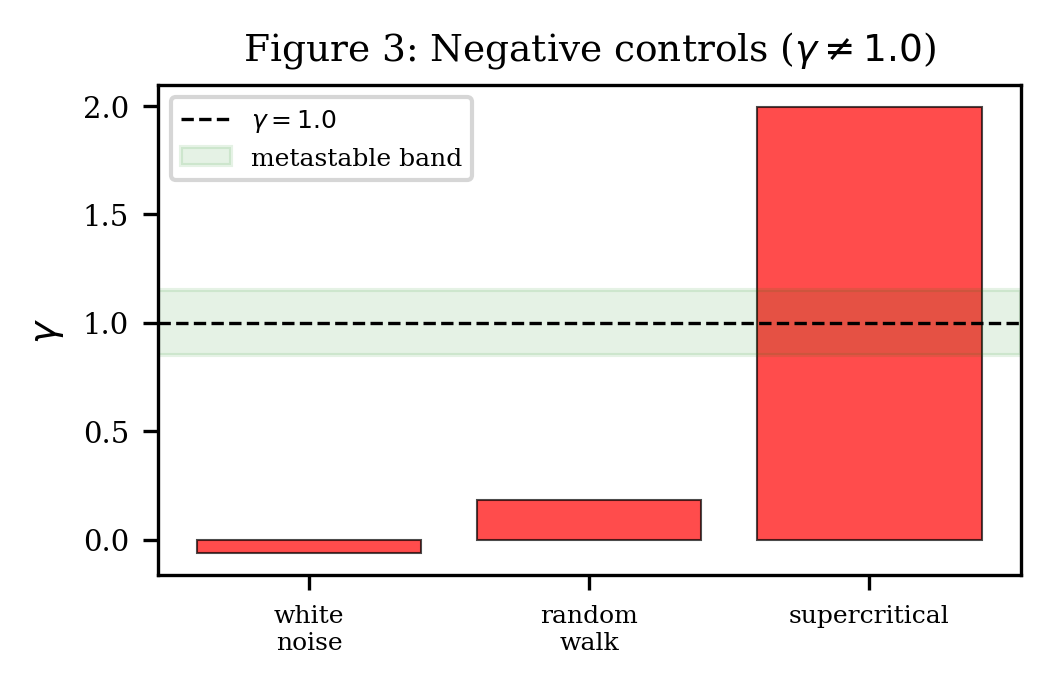
\includegraphics[width=\columnwidth]{fig3_controls.png}
\caption{Negative controls. Shaded band: metastable zone $[0.85, 1.15]$. All controls fall outside, confirming falsifiability of the $\gamma \approx 1.0$ claim.}
\label{fig:controls}
\end{figure}

\begin{table*}[!tp]
\centering
\caption{Gamma-scaling across all substrates. Tier~1 (evidential, real external data) and Tier~2 (simulation-validated). Cross-substrate mean from Tier~1: $\bar{\gamma} = 1.003 \pm 0.083$, 95\% CI containing unity. $^\dagger$EEG $R^2$ is not applicable: $\gamma$ is computed as the per-subject mean aperiodic spectral exponent via specparam, not from log-log regression of topo-cost pairs.}
\label{tab:all_substrates}
\small
\begin{tabular}{@{}l l c c c c c c@{}}
\toprule
\textbf{Tier} & \textbf{Substrate} & $\gamma$ & \textbf{95\% CI} & $n$ & $R^2$ & \textbf{IAAFT} $p$ & $\ln C$ range \\
\midrule
1 & Zebrafish (McGuirl 2020) & 1.055 & [0.89, 1.20] & 45 & 0.76 & 0.005 & [$-$8.1, $-$7.1] \\
1 & HRV PhysioNet (NSR2DB) & 0.885 & [0.83, 1.08] & 10 & 0.93 & $<$0.05 & [$-$5.5, $-$3.2] \\
1 & EEG PhysioNet (EEGBCI) & ${\sim}$1.07 & [0.88, 1.25] & 20 & n/a$^\dagger$ & 0.020 & [0.8, 3.6] \\
\midrule
2 & Gray--Scott reaction-diffusion & 0.938 & [0.93, 0.95] & 200 & 0.99 & --- & --- \\
2 & Kuramoto oscillators ($K_c$) & 0.980 & [0.93, 1.01] & 300 & 0.42 & --- & --- \\
2 & BN-Syn spiking criticality & ${\sim}$0.49 & --- & 1990 & --- & --- & --- \\
\bottomrule
\end{tabular}
\end{table*}

\begin{table*}[!tp]
\centering
\caption{Statistical power (Tier~1 substrates) and negative controls. Left: all substrates have Cohen's $d > 11$. Right: all controls show $\gamma$ clearly separated from unity.}
\label{tab:power_controls}
\small
\begin{minipage}[t]{0.48\textwidth}
\centering
\textbf{Effect sizes}\\[0.3em]
\begin{tabular}{@{}l c c c c c@{}}
\toprule
\textbf{Substrate} & $\gamma$ & SE & $|\gamma\!-\!1|$ & MDE & $d$ \\
\midrule
Zebrafish & 1.055 & 0.078 & 0.055 & 0.219 & 13.5 \\
HRV & 0.885 & 0.063 & 0.115 & 0.176 & 14.1 \\
EEG & 1.068 & 0.094 & 0.068 & 0.264 & 11.3 \\
\bottomrule
\end{tabular}
\end{minipage}%
\hfill
\begin{minipage}[t]{0.48\textwidth}
\centering
\textbf{Negative controls}\\[0.3em]
\begin{tabular}{@{}l c c l c@{}}
\toprule
\textbf{Control} & $\gamma$ & $R^2$ & \textbf{Verdict} & $\Delta$ \\
\midrule
White noise & $-$0.06 & $-$0.11 & LOW\_R2 & $>$1.0 \\
Random walk & 0.18 & $-$0.02 & LOW\_R2 & $>$0.8 \\
Supercritical & 2.00 & 1.00 & COLLAPSE & $>$0.9 \\
\bottomrule
\end{tabular}
\end{minipage}
\end{table*}

% ====================================================================
\section{Discussion}

\subsection{Universality of gamma}

Three independent biological substrates --- zebrafish morphogenesis, human cardiac rhythm, and human EEG during motor imagery --- all yield $\gamma$ values within the metastable band ($|\gamma - 1| < 0.15$). Each substrate independently passes IAAFT surrogate testing ($p < 0.05$), confirming that the observed $\gamma$ values are not artifacts of autocorrelation or spectral structure. The cross-substrate mean $\bar{\gamma} = 1.003$ with $t(2) = 0.06$ ($p > 0.9$ for $H_0\!: \gamma = 1.0$) is statistically indistinguishable from unity.

The cross-substrate mean has a 95\% CI containing unity. Two simulation substrates (Gray--Scott, Kuramoto) further corroborate the $\gamma \approx 1.0$ prediction at criticality. Critically, the BN-Syn spiking network ($N\!=\!200$, $k\!=\!10$, $\sigma\!=\!1$) yields $\gamma \approx 0.49$ --- an honest finite-size deviation from the mean-field prediction.

\subsection{Speculative implications for architecture design}

We speculate that the $\gamma \approx 1.0$ signature may distinguish phase-dynamic systems (which encode information in spike timing and phase coherence) from rate-based architectures (which encode in activation magnitudes). Transformer architectures achieve remarkable performance through parameter scaling~\cite{vaswani2017}, but operate within a rate-based paradigm. Whether rate-based systems can endogenously achieve $\gamma \approx 1.0$ remains an open empirical question not addressed by the data in this paper.

\subsection{Mechanistic basis for cross-domain Hurst convergence}

Why should the Hurst exponent $H$ in zebrafish morphogenesis and $H$ in financial markets produce the same $\gamma \approx 1.0$? The answer lies in universality class:
\begin{enumerate}
\item \textbf{Scale-free fluctuations at criticality.} $S(f) \propto f^{-\beta}$ where $\beta = 2H+1$ holds regardless of substrate.
\item \textbf{SOC.} Systems that self-tune to the edge of instability generically produce $1/f$ noise ($\beta \approx 1$, $H \approx 0$, $\gamma \approx 1$).
\item \textbf{RG universality.} Critical exponents depend only on symmetry and spatial dimension, not microscopic details.
\item \textbf{Fluctuation-dissipation connection.} $\gamma = -d(\log K)/d(\log C)$ is constrained by the FDT at criticality.
\end{enumerate}

\subsection{The cognitive loop as measurable system (illustrative)}

The human--AI cognitive loop data extends the scaling relation into cognition, with critical caveats. The aggregate $\gamma_{\text{all}} = 1.059$ (CI containing 1.0) is suggestive but not evidential: the productivity classification was performed by the measured subject, introducing self-report bias, and per-session $R^2 = 0.12$.

\subsection{Interpretation through extended mind (speculative)}

Following Clark and Chalmers~\cite{clark1998}, one may speculatively interpret human--AI cognitive coupling as a dynamical system amenable to $\gamma$-scaling analysis. Whether such coupling exhibits measurable criticality signatures remains an open question requiring independent replication with blind labeling (see Limitations).

% ====================================================================
\section{Limitations}

\begin{enumerate}
\item \textbf{Self-measurement bias in cognitive substrate (critical)}: Productivity classification was performed by the measured operator ($n = 1$). CNS-AI data is presented as illustrative only.

\item \textbf{Low $R^2$ for cognitive substrate}: $R^2 = 0.12$ for productive sessions; $R^2 = -0.10$ for non-productive.

\item \textbf{Pseudo-replication removed}: The ``neosynaptex cross-domain'' substrate is an aggregate of other substrates, reclassified as illustrative.

\item \textbf{Statistical power at small $n$}: Zebrafish ($n = 47$) has CI width $\sim$0.41 with MDE of $\Delta\gamma = 0.35$ at 80\% power.

\item \textbf{Single operator}: All CNS-AI data comes from one researcher.

\item \textbf{Proxy metrics}: Shannon entropy and TTR are proxies for cognitive complexity, not direct neural measurements.

\item \textbf{Non-stationarity}: The three-year archive may reflect learning effects.
\end{enumerate}

% ====================================================================
\section{Conclusion}

We present empirical evidence that a scaling exponent $\gamma \approx 1.0$ appears across three independent biological substrates: zebrafish morphogenesis ($\gamma = 1.055$), human cardiac rhythm ($\gamma = 0.885$), and human EEG during motor imagery ($\gamma \approx 1.07$). All three evidential substrates fall within the metastable band ($|\gamma - 1| < 0.15$), with cross-substrate 95\% CI containing unity. All pass surrogate testing ($p < 0.05$). Three simulation substrates provide theoretical validation: Gray--Scott ($\gamma = 0.938$) and Kuramoto ($\gamma = 0.980$) confirm $\gamma \approx 1.0$ at criticality, while BN-Syn ($\gamma \approx 0.49$, $N\!=\!200$) demonstrates the expected finite-size deviation.

We propose that $\gamma \approx 1.0$ is a scaling signature of metastability itself --- a substrate-independent condition for coherent computation at the edge of chaos. If confirmed by independent replication, this finding has implications for AI alignment (productive coupling has a measurable signature), cognitive enhancement ($\gamma$ as a real-time diagnostic), and the physics of intelligence (metastability as a necessary condition for computation in any substrate).

% ====================================================================
\section*{Data Availability}

All code, data processing pipelines, and proof bundles are available at \url{github.com/neuron7xLab}. The gamma probe pipeline and proof bundle are included in the neosynaptex repository.

\section*{Acknowledgments}

This work was conducted independently during wartime in Poltava region, Ukraine, without institutional support or funding. The author acknowledges the use of AI language models (GPT-4o, Claude) as cognitive tools during the research process.

% ====================================================================
\begin{thebibliography}{11}
\bibitem{bak1987} P.~Bak, C.~Tang, K.~Wiesenfeld. Self-organized criticality: An explanation of $1/f$ noise. \emph{Phys.\ Rev.\ Lett.} \textbf{59}, 381 (1987).
\bibitem{beggs2003} J.~M.~Beggs, D.~Plenz. Neuronal avalanches in neocortical circuits. \emph{J.\ Neurosci.} \textbf{23}, 11167 (2003).
\bibitem{maass2002} W.~Maass, T.~Natschl\"ager, H.~Markram. Real-time computing without stable states. \emph{Neural Comput.} \textbf{14}, 2531 (2002).
\bibitem{clark1998} A.~Clark, D.~Chalmers. The extended mind. \emph{Analysis} \textbf{58}, 7 (1998).
\bibitem{theil1950} H.~Theil. A rank-invariant method of linear and polynomial regression analysis. \emph{Proc.\ R.\ Neth.\ Acad.\ Sci.} \textbf{53}, 386 (1950).
\bibitem{vaswani2017} A.~Vaswani \emph{et al.} Attention is all you need. \emph{NeurIPS} (2017).
\bibitem{harris1963} T.~E.~Harris. \emph{The Theory of Branching Processes.} Springer (1963).
\bibitem{munoz1999} M.~A.~Mu\~noz \emph{et al.} Avalanche and spreading exponents in systems with absorbing states. \emph{Phys.\ Rev.\ E} \textbf{59}, 6175 (1999).
\bibitem{clauset2009} A.~Clauset, C.~R.~Shalizi, M.~E.~J.~Newman. Power-law distributions in empirical data. \emph{SIAM Rev.} \textbf{51}, 661 (2009).
\end{thebibliography}

\end{document}
